%%%%%%%%%%%%%%%%%%%%%%%%%%%%
% Prototype Implementation %
%%%%%%%%%%%%%%%%%%%%%%%%%%%%

\chapter{Prototyp-Implementierung}
\label{chapter:prototype}

Um den in Kapitel \ref{chapter:presented-approach} vorgestellten Ansatz für das interaktive Layout von Diagrammen und insbesondere die neu eingeführten Mechanismen für die Interaktion zu validieren, wurde im Rahmen der Bachelor-Arbeit ein Prototyp entwickelt. Mit der Beschreibung des Prototyps beschäftigt sich dieses Kapitel. In Abschnitt \ref{sec:technologies} wird auf die gewählten Technologien eingegangen. Die Benutzeroberfläche und die unterstützten Funktionen werden in Abschnitt \ref{sec:functions} vorgestellt. In Abschnitt \ref{sec:architecture} wird die Architektur des Prototyps thematisiert und es werden einzelnen Komponenten beschrieben. Schließlich folgt in Abschnitt \ref{sec:prototype-summary} eine Zusammenfassung.

\section{Technologie}
\label{sec:technologies}

Bevor die Entwicklung des Prototyps begonnen hat, wurde nach verfügbaren Komponenten gesucht, die in dem Prototyp verwendet werden könnten. Der umzusetzende Ansatz weist spezielle \textbf{Mechanismen für die Interaktion} auf (siehe Abschnitt \ref{sec:interaction-mechanisms}), die weder in kommerziellen Anwendungen noch in wissenschaftlichen Arbeiten gefunden wurden. Daher lässt sich für die Interaktion keine bestehende Software-Bibliothek einsetzen und die Umsetzung der Mechanismen der Interaktion bildet einen wesentlichen Teil der Entwicklung des Prototyps.

Des Weiteren wurde der Einsatz einer Bibliothek zum \textbf{Graphzeichnen} bedacht. Da die in diesen Bibliotheken bereitgestellte Algorithmen in der Regel eine automatische Berechnung des Layouts durchführen, ist eine Variierung des Layouts durch den Nutzer nicht möglich (siehe Abschnitt \ref{sec:automatic-layout}). Dies ist ebenfalls der Fall beim dem Einsatz dieser Algorithmen in interaktiven Ansätzen. Insbesondere in dem Pattern-basierten Ansatz aus \cite{Maier12A-Pattern-based} ist deutlich zu erkennen, dass sich das Layout nach der Anwendung eines Algorithmus zum Graphzeichnen auf einen gewählten Teil des Diagramms nicht modifizieren lässt (siehe Abschnitt \ref{subsubsec:pattern-based-approach}). Das Problem des statischen Verhaltens wurde ebenfalls in Bibliotheken für das \textbf{automatische Layout von Klassendiagrammen} festgestellt. Da die Möglichkeit der Layout-Variierung durch den Nutzer in dem präsentierten Ansatz eine große Bedeutung hat, wurde entschieden, die in Abschnitt \ref{subsec:concrete-layout-algorithms} beschriebene Layout-Algorithmen eigenständig zu implementieren. Da es sich um vereinfachte Algorithmen handelt, wurde der Einfachheit halber zu keinem \textbf{Constraintlöser} gegriffen, der z.B. in \textit{Dunnart} eingesetzt wird (siehe Abschnitt \ref{subsubsec:constraint-based-approaches}) und in Form der Software-Bibliothek \textit{Adaptagrams}\footnote{\url{https://github.com/mjwybrow/adaptagrams}} verfügbar ist. Der Einsatz eines Constraintlösers für einen verallgemeinerten Layout-Algorithmus wird in Abschnitt \ref{subsec:generalization-for-class-diagrams} diskutiert.

Es wäre denkbar, das \textbf{Layout-Framework aus \cite{Maier12A-Pattern-based}} als Grundlage für die Umsetzung des Prototyps einzusetzen. Dafür wäre es notwendig, die freie Positionierung einzuschränken, z.B. durch das Einführen von impliziten Layout-Patterns. Weiterhin müssten die in \cite{Maier12A-Pattern-based} vorgestellten allgemeinen Layout-Patterns zusammengefasst und um die Möglichkeit der Variierung erweitert werden. Schließlich müsste eine Unterstützung für die Mechanismen der Interaktion geschaffen werden. Da das Layout-Framework zu der Zeit der Anfertigung dieser Bachelor-Arbeit nicht veröffentlicht wurde, war sein Einsatz ausgeschlossen.

Aufgrund der Konzentration auf die Mechanismen der Interaktion und die Bestandteile der Layout-Berechnung wurde das bearbeitete Modell einfach gehalten. Dies wurde bereits in Abschnitt \ref{subsec:concrete-layout-algorithms} zur Vorstellung der konkreten Layout-Algorithmen beschrieben. Deshalb war es nicht notwendig, eine verfügbare Implementierung des \textbf{UML-Metamodells} (z.B. Ecore\footnote{\url{http://www.eclipse.org/modeling/emf}}) zu verwenden.

Da keine Komponenten wiederverwendet werden konnten, wurde eine komplett neue Desktop-Anwendung entwickelt. Es handelt sich um eine native \textbf{\textit{Mac OS X} Anwendung}, die in der Programmiersprache \textit{Objective-C} entwickelt wurde. Sie verwendet ausschließlich die Standardbibliotheken \textit{Cocoa} und \textit{Quartz} und besitzt keine weiteren Abhängigkeiten.

\section{Funktionen}
\label{sec:functions}

Der Ansatz für das interaktive und diagrammspezifische Layout von Diagrammen wurde in einem prototypischen Werkzeug für die Erstellung von einfachen Klassendiagrammen umgesetzt. Das Werkzeug unterstützt Klassen und Vererbungsrelationen und bietet somit die Möglichkeit, Vererbungshierarchien von Klassen zu modellieren.

Die Benutzeroberfläche des Werkzeugfensters ist in zwei rechteckige Bereiche aufgeteilt. Links befindet sich die Sidebar mit Bedienungselementen und rechts der Canvas, in dem das modellierte Diagramm abgebildet wird. Die Sidebar besteht aus einer Palette mit Icons für das Hinzufügen von Klassen und Vererbungsrelationen, einem Button für das Zurücksetzen des modellierten Diagramms und einer Auswahl des verwendeten Layout-Algorithmus. Die Benutzeroberfläche der Anwendung wird mit Hilfe eines Screenshots in Abbildung \ref{fig:prototype-screenshot} veranschaulicht.

\begin{figure}[hbt]
    \centering
    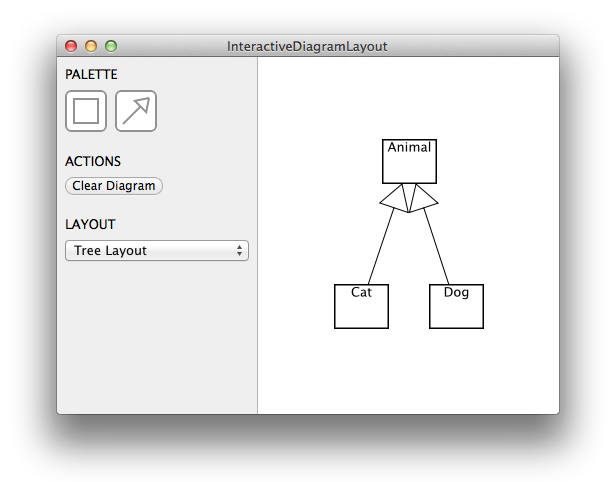
\includegraphics[scale=0.6]{assets/prototype-screenshot}
    \caption{Ein Screenshot des prototypischen Werkzeugs}
    \label{fig:prototype-screenshot}
\end{figure}

\subsection{Unterstützte Aktionen}
\label{subsec:supported-actions}

Der Prototyp unterstützt die grundlegenden Aktionen, die erforderlich sind, um ein Diagramm modellieren zu können. Insbesondere handelt es sich um die wichtigsten Bearbeitungsaktionen, die in Abschnitt \ref{subsec:edit-actions} vorgestellt wurden. Die einzelnen unterstützten Aktionen werden im Folgenden aufgelistet und kurz beschrieben:

\begin{itemize}

\item
\textbf{Hinzufügen einer Klasse}
Eine neue Klasse kann mit Hilfe von \enquote{Drag and Drop} dem Diagramm hinzugefügt werden, indem das linke Icon in der Palette angeklickt und in den Canvas gezogen wird. Nachdem der Mauszeiger den Canvas erreicht, wird die Klasse hinzugefügt, was durch einen Platzhalter gekennzeichnet wird. Danach wandelt die Aktion in eine Verschiebungsaktion um (siehe unten) und die Klasse kann an eine gewünschte Position verschoben werden.

\item
\textbf{Umbenennen einer Klasse}
Durch einen Doppelklick und das Eintragen eines Namens in das angezeigte Textfeld kann eine Klasse im Diagramm umbenannt werden. Aus zeitlichen Gründen konnte die Anpassung der Größe der Klassen nach der Änderung ihren Namen nicht implementiert werden.

\item
\textbf{Verschiebung einer Klasse}
Die Position einer Klasse im Diagramm kann durch den Nutzer geändert werden, indem die Klasse mit Hilfe des Mechanismus der temporären Schicht (siehe Abschnitt \ref{subsec:temporary-layer-mechanism}) verschoben wird. Dabei wird das Layout durch die ausgewählte Layout-Engine berechnet (siehe Abschnitt \ref{subsec:supported-layout-methods}).

\item
\textbf{Erzeugen einer Vererbungsrelation zwischen zwei Klassen}
Durch das Anklicken des rechten Icons in der Palette und das Ziehen eines Pfeils zwischen zwei Klassen im Diagramm wird eine Vererbungsrelation erstellt. Alternativ kann neben dem Anklicken des Icons auch die Taste \texttt{CTRL} gedrückt werden. Wenn der Nutzer versucht, eine semantisch ungültige Vererbungsrelation zu erstellen (z.B. einen Vererbungszyklus oder eine Mehrfachvererbung\footnote{Die Mehrfachvererbung ist ein gültiges Konstrukt in Klassendiagrammen der Notationssprache UML, wird aber in meisten objekt-orientierten Sprachen nicht unterstützt \cite{ArlowNeustadt05UML-2-and-the-Unified}. Für die Zwecke des Prototyps wird sie nicht zugelassen.}), wird eine Fehlermeldung angezeigt und der Vorgang bricht ab. Nachdem eine Vererbungsrelation erstellt wird und die ausgewählte Layout-Engine die Vererbungsrelationen unterstützt, wird das neu berechnete Layout auf das Diagramm angewendet.

\item
\textbf{Löschen des Inhalts}
Da das prototypische Werkzeug keine Möglichkeit der Auswahl von Objekten im Canvas bietet, wird weder das Löschen von Klassen noch von Relationen unterstützt. Um trotzdem das Zurücksetzen des Diagramms zu ermöglichen, gibt es für diese Funktion ein Button in der Sidebar.

\end{itemize}

Die Funktionsweise der beschriebenen Aktionen ist in einem Video unter dem Pfad \texttt{Proto\-type/Videos/Actions-Demo.mov} auf der eingereichten CD veranschaulicht.

Die implementierten Aktionen sind für die Validierung des umgesetzten Konzeptes und die Vorbereitung von Aufgaben für eine Nutzerstudie ausreichend, dennoch ist das prototypische Werkzeug nicht produktiv einsetzbar. Das liegt zum einen auf der starken Einschränkung der Notation der Klassendiagramme und zum anderen auf der ausschließlichen Unterstützung von grundlegenden Aktionen. Die möglichen Erweiterungen des Prototyps werden in Abschnitt \ref{subsec:extension-of-the-prototype} diskutiert.

\subsection{Unterstützte Layout-Methoden}
\label{subsec:supported-layout-methods}

Der Prototyp unterstützt beide konkreten Layout-Algorithmen aus Abschnitt \ref{subsec:concrete-layout-algorithms}, wobei der Algorithmus für das horizontale Layout als ein Zwischenschritt für die Implementierung des Algorithmus für das baumbasierte Layout dient und bei der Layout-Berechnung keine Relationen berücksichtigt.

Der aktuelle Algorithmus kann in der Sidebar ausgewählt werden und wird für die Layout-Berechnung im Diagramm verwendet. Außerdem wird bei der Änderung des Algorithmus ein initiales Layout berechnet, um das Layout des Diagramms in einen validen Zustand zu bringen (siehe Abschnitt \ref{subsec:concrete-layout-algorithms}). Für die Auswahl des Algorithmus können alternativ auch die Tastenkombinationen \texttt{CMD+1} und \texttt{CMD+2} genutzt werden.

\section{Architektur}
\label{sec:architecture}

Der Prototyp wurde in Form einer objekt-orientierten Anwendung implementiert und ist in vier logische Komponenten aufgeteilt: \textit{Layout Engine}, \textit{Dragging Manager}, \textit{Canvas View} und \textit{Application}. Die Abhängigkeiten zwischen den Hauptkomponenten sind in Abbildung \ref{fig:main-components} in Form eines Paketdiagramms dargestellt. Zu den Verantwortlichkeiten der Komponente \textit{Layout Engine} gehört u.a. die Beschreibung des Metamodells, die Verarbeitung der Nutzer-Aktionen und vor allem die Durchführung der Layout-Berechnung. Durch die Komponente \textit{Dragging Manager} wird eine abstrahierte Schnittstelle für die \enquote{Drag and Drop} Operation bereitgestellt. Die Darstellung und Interaktion mit dem Diagramm im Canvas wird in der Komponente \textit{Canvas View} realisiert. Schließlich werden die genannten Komponenten von der Komponente \textit{Application} zu einer lauffähigen Anwendung zusammengesetzt. Auf die wichtigsten Komponenten wird in den folgenden Abschnitten im Detail eingegangen.

\begin{figure}[hbt]
    \centering
    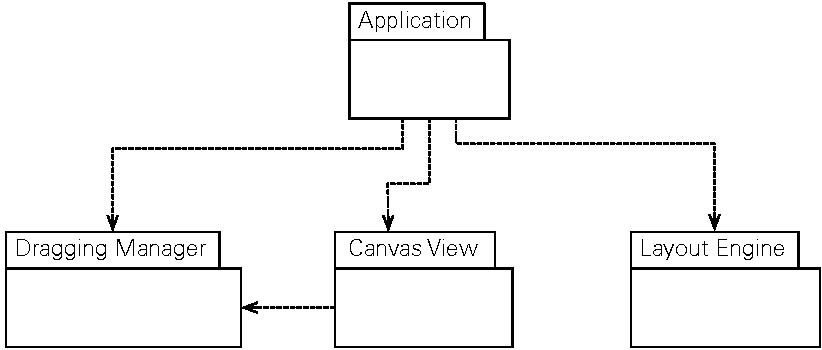
\includegraphics[scale=0.85]{assets/main-components}
    \caption{Eine Übersicht der grundlegenden Komponenten des Prototyps}
    \label{fig:main-components}
\end{figure}

\subsection{Layout Engine}

Die Komponente \textit{Layout Engine} bildet den wesentlichen Teil der Umsetzung des interaktiven Ansatzes aus dem Kapitel \ref{chapter:presented-approach}. Neben der Beschreibung der Layout-Eigenschaften und des Metamodells für die Diagramme verfügt diese Komponente über die Verwaltung von Layout-Patterns, Erstellung und Verarbeitung von Layout-Ereignissen und schließlich stellt sie die Funktion der Layout-Berechnung zur Verfügung. Aufgrund der Komplexität wurde \textit{Layout Engine} in folgende Unterkomponenten aufgeteilt: \textit{Geometry}, \textit{Diagram}, \textit{Layout}, \textit{Patterns}, \textit{Events} und \textit{Engines}. Eine Übersicht der Unterkomponenten und deren Beziehungen wird in Form eines Paketdiagramms in Abbildung \ref{fig:layout-engine-subcomponents} gegeben.

\begin{figure}[hbt]
    \centering
    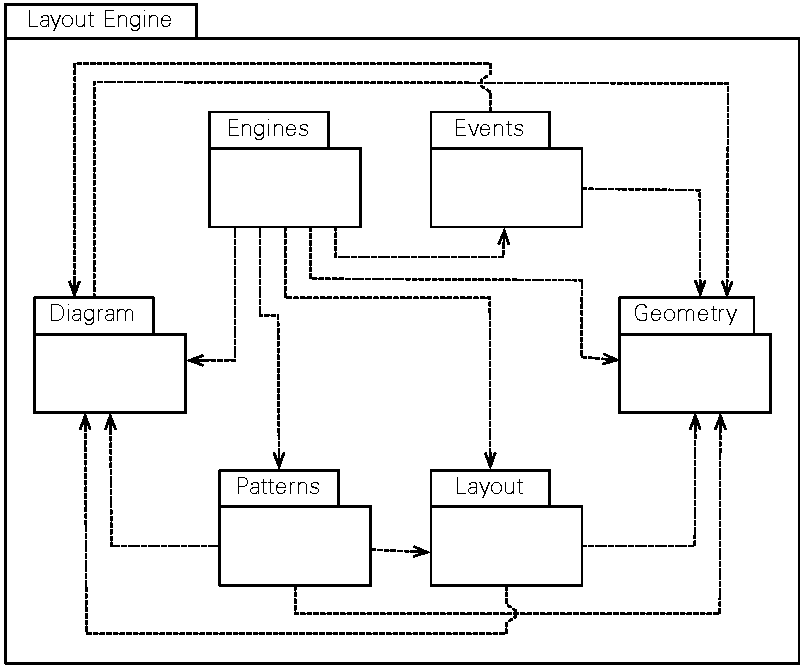
\includegraphics[scale=0.85]{assets/layout-engine-subcomponents}
    \caption{Eine Übersicht der Unterkomponenten der Komponente \textit{Layout Engine}}
    \label{fig:layout-engine-subcomponents}
\end{figure}

\subsubsection{Geometry}
\label{subsubsec:geometry}

Die Komponente \textit{Geometry} stellt die grundlegenden \textbf{geometrischen Datentypen} wie Punkt, Größe, Rechteck und Linie und für diese ausgelegte \textbf{geometrische Funktionen} bereit. Die neu eingeführten Datentypen unterscheiden sich von den entsprechenden Datentypen aus der Standardbibliothek wie \texttt{NSPoint}, \texttt{NSSize} und \texttt{NSRect} darin, dass die Werte in ganzen Zahlen angegeben werden und dass die Position des Rechtecks seinen Mittelpunkt darstellt. Durch die letztere Eigenschaft wird die Angabe der Positionen mit Hilfe des Mittelpunkts ermöglicht. Außerdem werden die Positionen in zentrierten Koordinaten angegeben, was die Umsetzung des impliziten Patterns zur Zentrierung des Diagramm-Inhalts fördert (siehe Abschnitt \ref{subsubsec:centering-of-diagram-content}) und die relative Layout-Berechnung vereinfacht. Da in \textit{Cocoa} und insbesondere in der für die grafische Repräsentation verantwortlichen Klasse \texttt{NSView} der Koordinatenursprung standardmäßig in der linken unteren Ecke liegt, war es notwendig eine Umrechnung der beiden Koordinatensysteme zu implementieren. In Abbildung \ref{fig:coordinates-conversion} ist der Sachverhalt illustriert, wobei die zentrierten Koordinaten blau und die Standardkoordinaten rot dargestellt sind. Die Zeichnung wird mit einem schwarzen Referenzrechteck eingeschlossen, das für die Umrechnung notwendig ist.

\begin{figure}[hbt]
    \centering
    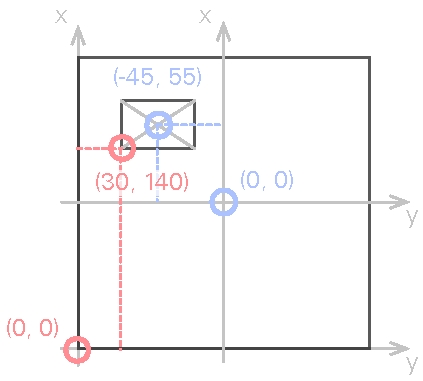
\includegraphics{assets/coordinates-conversion}
    \caption{Ein Beispiel der Koordinatenumrechnung für ein rechteckiges Objekt mit einer festen Größe}
    \label{fig:coordinates-conversion}
\end{figure}

\subsubsection{Diagram}
\label{subsubsec:component-diagram}

Das \textbf{Metamodell der Diagramme} ist ein Bestandteil der Komponente \textit{Diagram} und wird durch die Klassen \texttt{IDLDiagram}\footnote{Das Präfix \texttt{IDL} steht für den Projektnamen \textit{Interactive Diagram Layout} und wird in Objective-C Projekten für Klassen- und Funktionsnamen verwendet, um Namenskonflikte zu vermeiden.}, \texttt{IDLNode} und \texttt{IDLEdge} repräsentiert. Durch deren Instanziierung wird ein Modell eines Klassendiagramms mit Klassen und Vererbungsrelationen erstellt, was auch die Information über das aktuelle Layout kapselt, denn die Klasse \texttt{IDLNode} die Layout-Eigenschaft der Position besitzt.

Aus zeitlichen Gründen konnte diese Komponente nicht tiefgründig ausgearbeitet werden. Daher wird die abstrakte und konkrete Syntax der Elemente zusammengefasst und deren Semantik nur unvollständig unterstützt. Die mögliche Behebung dieser Schwachstelle wird in Abschnitt \ref{subsec:syntax-and-semantics-support-improvements} diskutiert.

\subsubsection{Layout}

Bei der Berechnung des Layouts ist es notwendig, die \textbf{Layout-Eigenschaften beschreiben} und auf ein Diagramm anwenden zu können. Diese Aufgaben übernimmt die Komponente \textit{Layout}, die die Klassen \texttt{IDLLayout} und \texttt{IDLLayoutApplier} zur Verfügung stellt. Die zuerst genannte Klasse beschreibt eine Abbildung von Klassen auf deren Positionen im Diagramm, ohne die eigentlichen Positionen der Klassen zu verändern. Weiterhin bietet sie die Möglichkeit der Layout-Komposition mit Hilfe einer relativen Zusammensetzung von mehreren Layouts. Um ein gegebenes Layout auf die abgebildeten Klassen anzuwenden, wird die zweitgenannte Klasse eingesetzt.

\subsubsection{Patterns}
\label{subsubsec:patterns}

Die Umsetzung der Layout-Patterns aus Abschnitt \ref{sec:layout-patterns} erfolgt auf zwei Wegen. Die impliziten Layout-Patterns werden nicht instanziiert und müssen von konkreten Layout-Engines eingehalten werden (siehe Abschnitt \ref{subsubsec:component-engines}). Dagegen werden von den expliziten Layout-Patterns Instanzen erstellt und in der Layout-Engine verwaltet. Zu diesem Zweck stellt die Komponente \textit{Patterns} zwei Klassen für \textbf{konkrete explizite Layout-Patterns}\footnote{Die implementierten expliziten Layout-Patterns unterstützen ausschließlich die Ausrichtungen, die für die Umsetzung der Layout-Algorithmen notwendig sind.} zur Verfügung, nämlich die Klasse \texttt{IDLAlignment\-Pat\-tern} für das Ausrichtungspattern und die Klasse \texttt{IDLTShapePattern} für das T-Shape-Pattern. Beide Klassen werden in einem Klassendiagramm\footnote{Da die Programmiersprache Objective-C spezielle Konstrukte aufweist, ist eine standardkonforme Abbildung von Objective-C Klassen in Klassendiagrammen der Notationssprache UML nicht möglich.} in Abbildung \ref{fig:layout-patterns-implementation} visualisiert.

\begin{figure}[hbt]
    \centering
    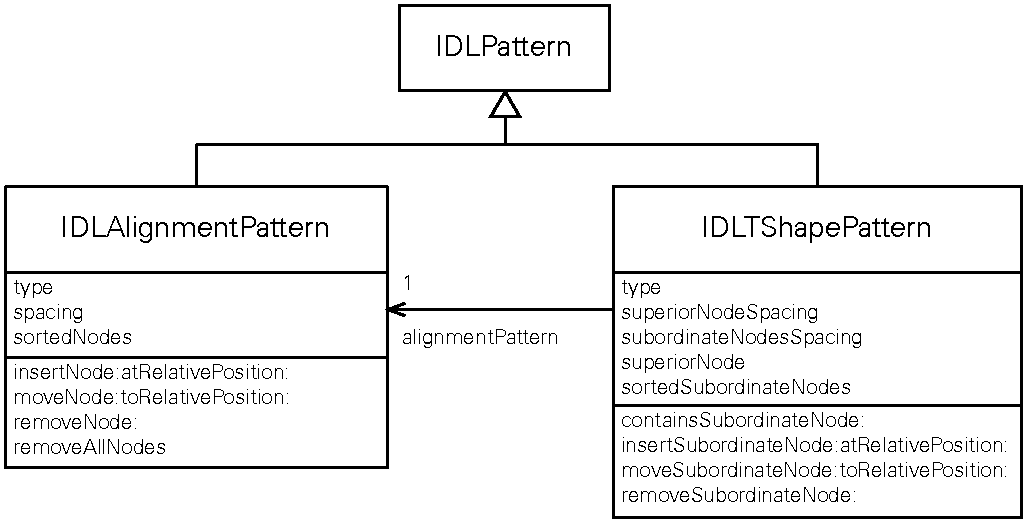
\includegraphics[scale=0.8]{assets/layout-patterns-implementation}
    \caption{Ein Klassendiagramm mit einer Übersicht der expliziten Layout-Patterns}
    \label{fig:layout-patterns-implementation}
\end{figure}

Die Klassen für die konkreten expliziten Layout-Patterns beschreiben ihre geometrischen Eigenschaften, ermöglichen die Verwaltung von verknüpften Knoten\footnote{Die Programmierschnittstellen im Prototyp verwenden die Begriffe \textit{Knoten} (engl.: \enquote{node}) und \textit{Kante} (engl.: \enquote{edge}) anstatt von \textit{Klasse} und \textit{Vererbungsrelation}.} und berechnen das relative Layout für diese. Weiterhin besitzen die Klassen Methoden für die Verschiebung von einem verknüpften Knoten an eine relative Position, um die Reihenfolge der Knoten zu verändern. Dadurch wird die Variierung der Layout-Patterns erreicht.

Ein weiterer interessanter Aspekt der implementierten Layout-Patterns ist die Möglichkeit ihrer Wiederverwendung und Komposition. Dem Klassendiagramm in Abbildung \ref{fig:layout-patterns-implementation} ist zu entnehmen, dass die Klasse \texttt{IDLShapePattern} intern eine Instanz der Klasse \texttt{IDLAlignmentPattern} verwendet. Diese ist für die Verwaltung der untergeordneten Knoten zuständig.

\subsubsection{Events}
\label{subsubsec:component-events}

Die Komponente \textit{Events} stellt Klassen für die \textbf{Beschreibung von Layout-Ereignissen} zur Verfügung, deren Konzept in Abschnitt \ref{sec:layout-calculation} erläutert wurde. Im Prototyp wurden die Layout-Ereignisse implementiert, die den unterstützten Bearbeitungsaktionen aus Abschnitt \ref{subsec:supported-actions} entsprechen. Alle Klassen für konkrete Layout-Ereignisse erben von der Klasse \texttt{IDLLayoutEvent} und sind in einem Klassendiagramm in Abbildung \ref{fig:layout-events-implementation} veranschaulicht.

\begin{figure}[hbt]
    \centering
    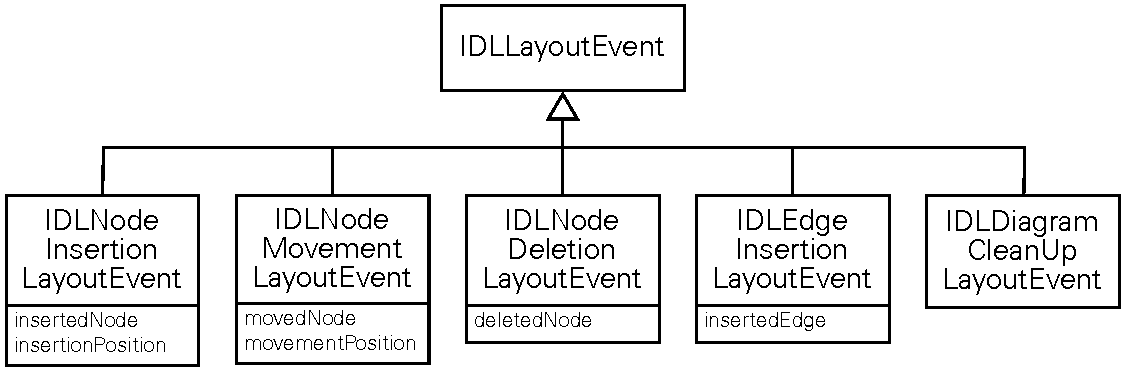
\includegraphics[scale=0.8]{assets/layout-events-implementation}
    \caption{Ein Klassendiagramm mit Übersicht der unterstützten Layout-Ereignisse}
    \label{fig:layout-events-implementation}
\end{figure}

Obwohl der Prototyp keine Möglichkeit des Löschens von einzelnen Knoten bietet, wird trotzdem das Layout-Ereignis \texttt{IDLNodeDeletionLayoutEvent} unterstützt. Es wird genau dann erzeugt und verarbeitet, wenn während der Hinzufügung eines Knotens der Mauszeiger außerhalb des Canvas bewegt wird. Dadurch wäre mit der Implementierung der Auswahl von einzelnen Knoten die Funktion des Löschens automatisch gewährleistet.

\subsubsection{Engines}
\label{subsubsec:component-engines}

Alle oben aufgeführten Komponenten werden durch die Komponente \textit{Engines} zusammengesetzt, um die eigentliche \textbf{Layout-Berechnung} zu realisieren. Zum einen verfügt die Komponente über eine abstrakte Klasse \texttt{IDLLayoutEngine} und zum anderen über zwei konkreten Unterklassen \texttt{IDLHorizontalLayoutEngine} und \texttt{IDLTreeLayoutEngine}, die die Layout-Algorithmen aus Abschnitt \ref{subsec:concrete-layout-algorithms} umsetzen. Wie bereits in Abschnitt \ref{subsec:supported-layout-methods} beschrieben wurde, kann die Layout-Engine zur Laufzeit des Prototyps gewählt werden.

Die konkreten Layout-Engines besitzen eine Referenz auf den Inhalt des Diagramms und müssen daher nach jeder Änderungen im Diagramm mit Hilfe von Layout-Ereignissen synchronisiert werden, um das Layout aktuell zu halten. Neben der Fähigkeit, alle Typen der Layout-Ereignisse aus Abschnitt \ref{subsubsec:component-events} zu verarbeiten, sind die Layout-Engines in der Lage, das initiale Layout zu berechnen, u.a. durch Instanziierung von expliziten Layout-Patterns, die in den Layout-Engines verwaltet werden. Die Klasse \texttt{IDLHorizontalLayoutEngine} besitzt nur eine Instanz des Ausrichtungspatterns. Dagegen werden in der Klasse \texttt{IDLTreeLayoutEngine} während der Laufzeit die Layout-Patterns dynamisch erzeugt und gelöscht. Bevor die Layout-Patterns verwendet werden können, müssen ihre geometrischen Parameter konfiguriert werden (siehe Abschnitte \ref{subsec:explicit-layout-patterns} und \ref{subsubsec:patterns}). Die in den Implementierungen der konkreten Algorithmen verwendete Werte wurden beispielhaft gewählt. Idealerweise sollten die passenden Werte für die Algorithmen anhand von geeigneten Methoden ermittelt und festgelegt werden, wobei es nicht ausgeschlossen wird, die Einstellung von einigen Eigenschaften des Algorithmus dem Nutzer zu überlassen, um den Algorithmus nach seinen Wünschen zu konfigurieren.

Das Layout wird in dem Algorithmus durch die Zusammensetzung der instanziierten Layout-Patterns berechnet. Dies ist nur dadurch möglich, weil die Algorithmen für die festgelegte Struktur der Diagramme angepasst sind. Der eventuelle Einsatz eines Constraintlösers und eine Verallgemeinerung der Layout-Algorithmen wird in Abschnitt \ref{subsec:generalization-for-class-diagrams} diskutiert.

\subsection{Canvas View}
\label{subsec:canvas-view}

Die Komponente \textit{Canvas View} wird in die Präsentationsschicht des Design Patterns \textit{Model View Controller} eingeordnet und ist für die \textbf{visuelle Repräsentation des Diagramms} und die \textbf{Interaktion im Canvas} zuständig. Den Kern dieser Komponente bildet die Klasse \texttt{IDLCanvas\-View}, die ihre Oberklasse \texttt{NSView} um die Möglichkeit des Zeichnens von Diagrammen erweitert. Dies wird mit Hilfe von der Zusammensetzung von Layer aus dem Framework \textit{Core Animation} realisiert. Die Informationen über die einzelnen Elemente und ihre Layout-Eigenschaften werden mittels des Delegate-Patterns abgefragt, so dass die Komponente vom Rest der Anwendung und insbesondere von der Layout-Berechnung abgekoppelt bleibt.

Obwohl die implementierten Layout-Engines ausschließlich die Positionen der Klassen berechnen, werden von \texttt{IDLCanvasView} alle Layout-Eigenschaften benötigt, um die Klassen und Vererbungsrelationen darstellen zu können, d.h. auch die Größe der Klassen und die Start- bzw. Endpunkte der Vererbungsrelationen. Im Prototyp wird einfachheitshalber die Größe der Klassen konstant gehalten und die Start- bzw. Endpunkte ähnlich wie in \textit{OmniGraffle} (siehe Abschnitt \ref{subsubsec:connection-points}) anhand der Eigenschaften der verbundenen Klassen außerhalb dieser Komponente berechnet. Da der Koordinatenursprung in \texttt{IDLCanvasView} in der linken unteren Ecke liegt, müssen alle Koordinaten zuerst umgerechnet werden (siehe Abschnitt \ref{subsubsec:geometry}). Wenn die Größe des Fensters geändert wird, erfolgt die Umrechnung erneut, so dass der Inhalt des Diagramms stets zentriert bleibt.

Die Interaktion mit dem Canvas besteht in der Ausführung von Bearbeitungsaktionen, die in dieser Komponente aus der Eingabe durch die Maus und Tastatur gebildet werden. Die Anwendung wird über die Ausführung jeder Bearbeitungsaktion informiert und erzeugt für sie ein oder mehrere Layout-Ereignisse. Diese werden anschließend an die Layout-Engine übergegeben. Sobald sich das Layout des Diagramms in der Layout-Engine ändert, wird darüber \textit{Canvas View} benachrichtigt, was zum Auslösen eines Layout-Übergangs führt. Wie bereits in Abschnitt \ref{subsec:layout-transitions} beschrieben wurde, wird an dieser Stelle eine Animation eingesetzt. Konkret handelt es sich um die implizite Animation der Properties der Layer, die durch das Framework \textit{Core Animation} bereitgestellt wird. Um die Animation flüssiger zu gestalten, wäre es denkbar, fortgeschrittene Mechanismen der Animation wie z.B. das Animations-Framework POP\footnote{\url{https://github.com/facebook/pop}} einzusetzen.

\section{Zusammenfassung}
\label{sec:prototype-summary}

Das in Kapitel \ref{chapter:presented-approach} entworfene Konzept für das Layout von Diagrammen wurde in Form eines Werkzeugs zur Erstellung von vereinfachten Klassendiagrammen prototypisch umgesetzt.

Es handelt sich um eine objekt-orientierte Anwendung für das Betriebsystem \textit{Mac OS X}, die in der Programmiersprache \textit{Objective-C} geschrieben ist. Da in der Vorbereitungsphase festgestellt wurde, dass für die Umsetzung des Konzeptes keine bestehende Bibliothek eingesetzt werden kann, wurde entschieden, eine ganz neue Anwendung zu implementieren. Diese verwendet ausschließlich die Standardbibliotheken der Mac Plattform. Der Quellcode sowie die kompilierte Version der Anwendung sind auf der beigelegten CD zu finden (für die konkreten Pfade siehe Abschnitt \ref{sec:cd-content-prototype}).

Das implementierte Werkzeug unterstützt Basisfunktionen, die für die Erstellung und Bearbeitung eines vereinfachten Klassendiagramms notwendig sind. Dies ermöglicht das praktische Testen des vorgestellten Konzeptes in einem wirklichkeitsnahen Anwendungsfall. Dennoch konnten in der initialen Version des Prototyps viele nützliche Funktionen aus zeitlichen Gründen nicht implementiert werden. Des Weiteren wurden in dem Prototyp beide konkreten Algorithmen aus Abschnitt \ref{subsec:concrete-layout-algorithms} umgesetzt, zwischen den zur Laufzeit umgeschaltet werden kann.

Während der Entwicklung der Anwendung wurde auf eine saubere architektonische Trennung geachtet. Die Architektur ist in mehrere Komponenten aufgeteilt, deren Abhängigkeiten untereinander minimiert sind. Insbesondere ist die Layout-Berechnung in der Komponente \textit{Layout Engine} von dem Rest der Anwendung gekapselt und in weitere Unterkomponenten aufgeteilt. Die entworfene Mechanismen der Interaktion wurden in der Komponente \textit{Canvas View} umgesetzt. Eine detaillierte Beschreibung der Architektur kann in diesem Kapitel nachgelesen werden.

Der wesentliche Teil des entworfenen Konzeptes konnte erfolgreich in dem Prototyp umgesetzt werden. Mit einer gründlichen Evaluation beschäftigt sich allerdings das Kapitel \ref{chapter:evaluation}. Unter anderem werden in dem Kapitel Ergebnisse einer Nutzerstudie präsentiert, für die der implementierte Prototyp die Grundlage bildet.
